% answers.tex —— 2020 年·全国Ⅱ卷·理科 · 参考答案与详细解析片段
% 由 tools/generate_projects.py 依来源总账自 2020/2020_数学真题_全国2理_试题.md + 2020/2020_数学真题_全国2理_解析正文.md + 2020/2020_数学真题_全国2理_答案要点.md 生成，勿手改（改源 MD 后重跑）


\begin{answer}
\gksolhead{1}{}

\textbf{题目}：

已知集合 $U=\{-2,-1,0,1,2,3\}$，$A=\{-1,0,1\}$，$B=\{1,2\}$，则 $\complement_U(A\cup B)=$\mbox{（　　）}

（A）$\{-2,3\}$；（B）$\{-2,2,3\}$；（C）$\{-2,-1,0,3\}$；（D）$\{-2,-1,0,2,3\}$。

\Needspace{4\baselineskip}
\textbf{解析}

\Needspace{5\baselineskip}
先求并集：
\nopagebreak[4]
\[A\cup B=\{-1,0,1\}\cup\{1,2\}=\{-1,0,1,2\}.\]
\Needspace{5\baselineskip}
在全集 $U=\{-2,-1,0,1,2,3\}$ 中除去 $-1$，$0$，$1$，$2$，只剩 $-2$ 与 $3$，故
\nopagebreak[4]
\[\complement_U(A\cup B)=\{-2,3\}.\]

选 A。

\gkanswer{答案：A。$A\cup B=\{-1,0,1,2\}$，故 $\complement_U(A\cup B)=\{-2,3\}$。}

\end{answer}
\begin{answer}
\gksolhead{2}{}

\textbf{题目}：

若 $\alpha$ 为第四象限角，则\mbox{（　　）}

（A）$\cos2\alpha>0$；（B）$\cos2\alpha<0$；（C）$\sin2\alpha>0$；（D）$\sin2\alpha<0$。

\Needspace{4\baselineskip}
\textbf{解析}

\Needspace{5\baselineskip}
$\alpha$ 为第四象限角，即
\nopagebreak[4]
\[\alpha\in\left(2k\pi+\frac{3\pi}2,\ 2k\pi+2\pi\right)\quad(k\in\mathbf Z),\]
\Needspace{5\baselineskip}
于是
\nopagebreak[4]
\[\sin\alpha<0,\qquad \cos\alpha>0 .\]
\Needspace{5\baselineskip}
由二倍角公式
\nopagebreak[4]
\[\sin2\alpha=2\sin\alpha\cos\alpha<0,\]
故 D 恒成立。

另外三项都不恒成立：$\cos2\alpha=2\cos^2\alpha-1$ 的符号取决于 $\cos^2\alpha$ 与 $\dfrac12$ 的大小，例如 $\alpha=-\dfrac\pi6$ 时 $\cos2\alpha=\dfrac12>0$，而 $\alpha=-\dfrac\pi3$ 时 $\cos2\alpha=-\dfrac12<0$，故（A）（B）都不对；（C）与上式矛盾。

选 D。

\gkanswer{答案：D。$\alpha$ 为第四象限角给出 $\sin\alpha<0<\cos\alpha$，故 $\sin2\alpha=2\sin\alpha\cos\alpha<0$。}

\end{answer}
\begin{answer}
\gksolhead{3}{}

\textbf{题目}：

在新冠肺炎疫情防控期间，某超市开通网上销售业务，每天能完成 $1200$ 份订单的配货，由于订单量大幅增加，导致订单积压。为解决困难，许多志愿者踊跃报名参加配货工作。已知该超市某日积压 $500$ 份订单未配货，预计第二天的新订单超过 $1600$ 份的概率为 $0.05$。志愿者每人每天能完成 $50$ 份订单的配货，为使第二天完成积压订单及当日订单的配货的概率不小于 $0.95$，则至少需要志愿者\mbox{（　　）}

（A）$10$ 名；（B）$18$ 名；（C）$24$ 名；（D）$32$ 名。

\Needspace{4\baselineskip}
\textbf{解析}

\Needspace{5\baselineskip}
设至少需要 $n$ 名志愿者，则第二天该超市的日配货能力为
\nopagebreak[4]
\[1200+50n\ \text{（\text{份}）}.\]
\Needspace{5\baselineskip}
第二天需要配货的总量为「积压 $500$ 份」与「当日新订单」之和。由题意
\nopagebreak[4]
\[P(\text{\text{新订单}}\leqslant1600)=1-0.05=0.95,\]
\Needspace{5\baselineskip}
故只要
\nopagebreak[4]
\[1200+50n\geqslant500+1600=2100\]
\Needspace{5\baselineskip}
就能以不小于 $0.95$ 的概率在当天完成全部配货。解得
\nopagebreak[4]
\[50n\geqslant900,\qquad n\geqslant18 .\]
\Needspace{5\baselineskip}
反过来，$n=17$ 时配货能力只有 $2050$ 份，要当天配完必须「新订单 $\leqslant1550$ 份」；而
\nopagebreak[4]
\[P(\text{\text{新订单}}\leqslant1550)\leqslant P(\text{\text{新订单}}\leqslant1600)=0.95,\]
故完成概率达不到 $0.95$，$17$ 名不够。所以至少需要 $18$ 名志愿者。

选 B。

\gkanswer{答案：B。需日配货能力 $1200+50n\geqslant500+1600=2100$，即 $n\geqslant18$。}

\end{answer}
\begin{answer}
\gksolhead{4}{}

\textbf{题目}：

北京天坛的圜丘坛为古代祭天的场所，分上、中、下三层。上层中心有一块圆形石板（称为天心石），环绕天心石砌 $9$ 块扇面形石板构成第一环，向外每环依次增加 $9$ 块，下一层的第一环比上一层的最后一环多 $9$ 块，向外每环依次也增加 $9$ 块。已知每层环数相同，且下层比中层多 $729$ 块，则三层共有扇面形石板（不含天心石）\mbox{（　　）}

（A）$3699$ 块；（B）$3474$ 块；（C）$3402$ 块；（D）$3339$ 块。

\Needspace{4\baselineskip}
\textbf{解析}

\Needspace{5\baselineskip}
设每层有 $n$ 环。按题意，三层各环的石板数依次排成一个首项为 $9$、公差为 $9$ 的等差数列：
\nopagebreak[4]
\[9,\ 18,\ \cdots,\ 9n\ \big|\ 9(n+1),\ \cdots,\ 9\cdot2n\ \big|\ 9(2n+1),\ \cdots,\ 9\cdot3n .\]
\Needspace{5\baselineskip}
下层比中层多
\nopagebreak[4]
\[\sum_{k=2n+1}^{3n}9k-\sum_{k=n+1}^{2n}9k
=9\left[\frac{(2n+1+3n)n}2-\frac{(n+1+2n)n}2\right]
=9\cdot\frac{2n^2}{2}=9n^2 .\]
由 $9n^2=729$ 得 $n^2=81$，即 $n=9$。

\Needspace{5\baselineskip}
三层石板总数就是 $9,18,\cdots,9\cdot27$ 之和：
\nopagebreak[4]
\[9\cdot\frac{27\times28}{2}=9\times378=3402 .\]

选 C。

\gkanswer{答案：C。设每层 $n$ 环，下层比中层多 $9n^2=729$，得 $n=9$，三层共 $\dfrac{9\times9\times(9\times9+3)}2=3402$ 块。}

\end{answer}
\begin{answer}
\gksolhead{5}{}

\textbf{题目}：

若过点 $(2,1)$ 的圆与两坐标轴都相切，则圆心到直线 $2x-y-3=0$ 的距离为\mbox{（　　）}

（A）$\dfrac{\sqrt5}5$；（B）$\dfrac{2\sqrt5}5$；（C）$\dfrac{3\sqrt5}5$；（D）$\dfrac{4\sqrt5}5$。

\Needspace{4\baselineskip}
\textbf{解析}

圆与两坐标轴都相切，故圆心坐标为 $(t,t)$、$(t,-t)$、$(-t,t)$、$(-t,-t)$ 之一（$t\neq0$），半径为 $|t|$。

\Needspace{5\baselineskip}
若圆心为 $(t,t)$，由圆过 $(2,1)$ 得
\nopagebreak[4]
\[(2-t)^2+(1-t)^2=t^2\ \Longrightarrow\ t^2-6t+5=0\ \Longrightarrow\ t=1\ \text{\text{或}}\ t=5 .\]
\Needspace{5\baselineskip}
若圆心为 $(t,-t)$，则
\nopagebreak[4]
\[(2-t)^2+(1+t)^2=t^2\ \Longrightarrow\ t^2-2t+5=0,\]
判别式 $4-20<0$，无解；圆心为 $(-t,t)$ 时同理得 $t^2+2t+5=0$，亦无解；圆心为 $(-t,-t)$ 时圆在第三象限，不可能过第一象限的点 $(2,1)$。

\Needspace{5\baselineskip}
所以圆心只能是 $(1,1)$ 或 $(5,5)$。圆心到直线 $2x-y-3=0$ 的距离为
\nopagebreak[4]
\[d=\frac{|2t-t-3|}{\sqrt{2^2+(-1)^2}}=\frac{|t-3|}{\sqrt5},\]
\Needspace{5\baselineskip}
代入 $t=1$ 与 $t=5$ 都得
\nopagebreak[4]
\[d=\frac{2}{\sqrt5}=\frac{2\sqrt5}5 .\]

选 B。

\gkanswer{答案：B。圆心为 $(1,1)$ 或 $(5,5)$，二者到 $2x-y-3=0$ 的距离同为 $\dfrac{2}{\sqrt5}=\dfrac{2\sqrt5}5$。}

\end{answer}
\begin{answer}
\gksolhead{6}{}

\textbf{题目}：

数列 $\{a_n\}$ 中，$a_1=2$，$a_{m+n}=a_ma_n$。若 $a_{k+1}+a_{k+2}+\cdots+a_{k+10}=2^{15}-2^5$，则 $k=$\mbox{（　　）}

（A）$2$；（B）$3$；（C）$4$；（D）$5$。

\Needspace{4\baselineskip}
\textbf{解析}

\Needspace{5\baselineskip}
在 $a_{m+n}=a_ma_n$ 中取 $m=1$，得 $a_{n+1}=a_1a_n=2a_n$，又 $a_1=2$，故
\nopagebreak[4]
\[a_n=2^n\quad(n\in\mathbf N^*).\]
\Needspace{5\baselineskip}
所给等式左端是等比数列连续 $10$ 项之和：
\nopagebreak[4]
\[\sum_{i=k+1}^{k+10}2^i=2^{k+1}\cdot\frac{2^{10}-1}{2-1}=2^{k+1}(2^{10}-1).\]
\Needspace{5\baselineskip}
而
\nopagebreak[4]
\[2^{15}-2^5=2^5(2^{10}-1)=32(2^{10}-1).\]
比较得 $2^{k+1}=32=2^5$，即 $k+1=5$，$k=4$。

选 C。

\gkanswer{答案：C。由 $a_{m+n}=a_ma_n$ 得 $a_n=2^n$，所求和为 $2^{k+1}(2^{10}-1)=2^5(2^{10}-1)$，故 $k=4$。}

\end{answer}
\begin{answer}
\gksolhead{7}{}

\textbf{题目}：

如图是一个多面体的三视图，这个多面体某条棱的一个端点在正视图中对应的点为 $M$，在俯视图中对应的点为 $N$，则该端点在侧视图中对应的点为\mbox{（　　）}

（A）$E$；（B）$F$；（C）$G$；（D）$H$。
\nopagebreak[4]
\begin{center}% 2020 全国Ⅱ卷 理7：多面体的三视图
% 来源 PDF：普通高考/2020/2020全国2理(…).pdf 第 1 页（A3 横排），印面 1121，第 7 题右侧
% 结构：正视图为两块全等长方形（宽 1、高 1.19）上下错开 0.349 拼成，拐角处标 M；
%       侧视图为深 0.853、高 1.539 的矩形，被 y=1.19 与 y=0.349 两条水平线分成三带，
%       中带四角标 E（左上）、F（右上）、G（左下）、H（右下）；
%       俯视图为 2×1 的矩形，被中线分为两个正方形，中线上端标 N。
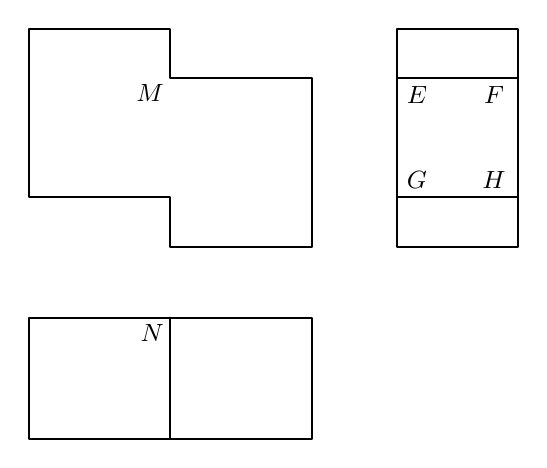
\begin{tikzpicture}[line width=0.7pt, font=\small,
  x=1.8cm, y=1.8cm, line cap=round, line join=round]
  % 尺寸：块宽 1，块高 1.19，块深 0.853，上下错开 0.349
  \def\hh{1.19}
  \def\dd{0.853}
  \def\oo{0.349}
  \def\gt{1.539}

  % 正视图
  \draw (0,\gt) -- (1,\gt) -- (1,\hh) -- (2,\hh) -- (2,0) -- (1,0) -- (1,\oo) -- (0,\oo) -- cycle;
  \node[below left, inner sep=2pt] at (1,\hh) {$M$};

  % 侧视图（左边缘 x=2.6）
  \begin{scope}[shift={(2.6,0)}]
    \draw (0,0) rectangle (\dd,\gt);
    \draw (0,\hh) -- (\dd,\hh);
    \draw (0,\oo) -- (\dd,\oo);
    \node at (0.14,\hh-0.12) {$E$};
    \node at (\dd-0.17,\hh-0.12) {$F$};
    \node at (0.14,\oo+0.12) {$G$};
    \node at (\dd-0.17,\oo+0.12) {$H$};
  \end{scope}

  % 俯视图（上边缘 y=-0.5）
  \begin{scope}[shift={(0,-0.5)}]
    \draw (0,0) rectangle (2,-\dd);
    \draw (1,0) -- (1,-\dd);
    \node[below left, inner sep=2pt] at (1,0) {$N$};
  \end{scope}
\end{tikzpicture}
\end{center}
\nopagebreak[4]
\Needspace{4\baselineskip}
\textbf{解析}

三视图给出同一多面体在三个方向上的投影：正视图给出「宽—高」，俯视图给出「宽—深」，侧视图给出「深—高」。

由正视图可见多面体由两个等宽的长方体拼接而成：左块占上层、右块占下层，两块在高度上错开一段，正视图中那个向内拐的角就是错开的分界高度，标号 $M$ 正落在这个角上。因此该端点 $P$ 的高度就是两块的公共分界高度，也就是侧视图中「上带与中带之间」的那条水平分界线所在的高度。

由俯视图可见整体水平投影是一个 $2\times1$ 的矩形，被中线（两块公共侧棱的投影）分成左右两个正方形；$N$ 标在这条中线的上端，故 $P$ 在深度方向取后端点。

侧视图以水平方向表示深度、竖直方向表示高度，且按规定左边对应物体的后方、右边对应物体的前方。于是 $P$ 位于侧视图的中带，高度在中带的上边界，深度取后端，即中带的左上角，对应点 $E$。

选 A。

\gkanswer{答案：A。该端点在正视图中位于层间分界高度，在俯视图中位于后缘，故在侧视图中对应中带的左上角 $E$。}

\end{answer}
\begin{answer}
\gksolhead{8}{}

\textbf{题目}：

设 $O$ 为坐标原点，直线 $x=a$ 与双曲线 $C:\dfrac{x^2}{a^2}-\dfrac{y^2}{b^2}=1$（$a>0$，$b>0$）的两条渐近线分别交于 $D$，$E$ 两点。若 $\triangle ODE$ 的面积为 $8$，则 $C$ 的焦距的最小值为\mbox{（　　）}

（A）$4$；（B）$8$；（C）$16$；（D）$32$。

\Needspace{4\baselineskip}
\textbf{解析}

\Needspace{5\baselineskip}
双曲线 $\dfrac{x^2}{a^2}-\dfrac{y^2}{b^2}=1$ 的两条渐近线为
\nopagebreak[4]
\[y=\frac ba x,\qquad y=-\frac ba x .\]
\Needspace{5\baselineskip}
令 $x=a$，得 $y=\pm b$，故
\nopagebreak[4]
\[D(a,b),\qquad E(a,-b),\]
\Needspace{5\baselineskip}
从而 $|DE|=2b$，原点 $O$ 到直线 $x=a$ 的距离为 $a$，于是
\nopagebreak[4]
\[S_{\triangle ODE}=\frac12\cdot 2b\cdot a=ab=8 .\]
\Needspace{5\baselineskip}
设半焦距为 $c$，则 $c^2=a^2+b^2$，由基本不等式
\nopagebreak[4]
\[2c=2\sqrt{a^2+b^2}\geqslant2\sqrt{2ab}=2\sqrt{16}=8,\]
等号当且仅当 $a=b=2\sqrt2$ 时成立（此时 $c=4$，$2c=8$ 确实可取到）。故焦距的最小值为 $8$。

选 B。

\gkanswer{答案：B。$D(a,b)$，$E(a,-b)$，面积 $ab=8$，焦距 $2c=2\sqrt{a^2+b^2}\geqslant2\sqrt{2ab}=8$。}

\end{answer}
\begin{answer}
\gksolhead{9}{}

\textbf{题目}：

设函数 $f(x)=\ln|2x+1|-\ln|2x-1|$，则 $f(x)$\mbox{（　　）}

（A）是偶函数，且在 $\left(\dfrac12,+\infty\right)$ 单调递增；（B）是奇函数，且在 $\left(-\dfrac12,\dfrac12\right)$ 单调递减；（C）是偶函数，且在 $\left(-\infty,-\dfrac12\right)$ 单调递增；（D）是奇函数，且在 $\left(-\infty,-\dfrac12\right)$ 单调递减。

\Needspace{4\baselineskip}
\textbf{解析}

\Needspace{5\baselineskip}
定义域为 $\left\{x\mid x\neq\pm\dfrac12\right\}$，关于原点对称，且
\nopagebreak[4]
\[f(-x)=\ln|-2x+1|-\ln|-2x-1|=\ln|2x-1|-\ln|2x+1|=-f(x),\]
故 $f$ 是奇函数，（A）（C）排除。

\Needspace{5\baselineskip}
在 $\left(-\infty,-\dfrac12\right)$ 上有 $2x+1<0$、$2x-1<0$，于是
\nopagebreak[4]
\[f(x)=\ln\frac{-(2x+1)}{-(2x-1)}=\ln\frac{2x+1}{2x-1}
=\ln\left(1+\frac{2}{2x-1}\right).\]
\Needspace{5\baselineskip}
记 $\varphi(x)=1+\dfrac{2}{2x-1}$，则
\nopagebreak[4]
\[\varphi'(x)=-\frac{4}{(2x-1)^2}<0\quad\left(x<-\frac12\right),\]
故 $\varphi$ 在 $\left(-\infty,-\dfrac12\right)$ 上单调递减，而 $\ln$ 单调递增，所以 $f$ 在 $\left(-\infty,-\dfrac12\right)$ 上单调递减。

\Needspace{5\baselineskip}
再核对（B）：在 $\left(-\dfrac12,\dfrac12\right)$ 上 $2x+1>0>2x-1$，
\nopagebreak[4]
\[f(x)=\ln\frac{2x+1}{1-2x},\]
其中 $\dfrac{2x+1}{1-2x}$ 的导数为 $\dfrac{4}{(1-2x)^2}>0$，$f$ 在此区间单调递增，故（B）错。

选 D。

\gkanswer{答案：D。$f$ 为奇函数，且在 $\left(-\infty,-\dfrac12\right)$ 上 $f(x)=\ln\left(1+\dfrac{2}{2x-1}\right)$ 单调递减。}

\end{answer}
\begin{answer}
\gksolhead{10}{}

\textbf{题目}：

已知 $\triangle ABC$ 是面积为 $\dfrac{9\sqrt3}4$ 的等边三角形，且其顶点都在球 $O$ 的球面上。若球 $O$ 的表面积为 $16\pi$，则 $O$ 到平面 $ABC$ 的距离为\mbox{（　　）}

（A）$\sqrt3$；（B）$\dfrac32$；（C）$1$；（D）$\dfrac{\sqrt3}2$。

\Needspace{4\baselineskip}
\textbf{解析}

\Needspace{5\baselineskip}
设等边三角形的边长为 $a$，则
\nopagebreak[4]
\[\frac{\sqrt3}4a^2=\frac{9\sqrt3}4\ \Longrightarrow\ a^2=9,\qquad a=3 .\]
\Needspace{5\baselineskip}
等边三角形外接圆半径
\nopagebreak[4]
\[r=\frac{a}{2\sin60^\circ}=\frac{3}{\sqrt3}=\sqrt3 .\]
球 $O$ 的表面积 $4\pi R^2=16\pi$，故球半径 $R=2$。

\Needspace{5\baselineskip}
设球心 $O$ 到平面 $ABC$ 的距离为 $d$，由球的截面性质，截面圆半径即为 $\triangle ABC$ 的外接圆半径，且
\nopagebreak[4]
\[R^2=r^2+d^2,\]
\Needspace{5\baselineskip}
故
\nopagebreak[4]
\[d=\sqrt{R^2-r^2}=\sqrt{4-3}=1 .\]

选 C。

\gkanswer{答案：C。边长 $3$，外接圆半径 $\sqrt3$，球半径 $2$，故距离 $\sqrt{2^2-(\sqrt3)^2}=1$。}

\end{answer}
\begin{answer}
\gksolhead{11}{}

\textbf{题目}：

若 $2^x-2^y<3^{-x}-3^{-y}$，则\mbox{（　　）}

（A）$\ln(y-x+1)>0$；（B）$\ln(y-x+1)<0$；（C）$\ln|x-y|>0$；（D）$\ln|x-y|<0$。

\Needspace{4\baselineskip}
\textbf{解析}

\Needspace{5\baselineskip}
把不等式移项：
\nopagebreak[4]
\[2^x-3^{-x}<2^y-3^{-y}.\]
\Needspace{5\baselineskip}
令
\nopagebreak[4]
\[h(t)=2^t-3^{-t},\]
\Needspace{5\baselineskip}
则
\nopagebreak[4]
\[h'(t)=2^t\ln2+3^{-t}\ln3>0,\]
\Needspace{5\baselineskip}
故 $h$ 在 $\mathbf R$ 上严格递增。于是原不等式等价于
\nopagebreak[4]
\[x<y,\qquad\text{\text{即}}\quad y-x>0 .\]
\Needspace{5\baselineskip}
因此
\nopagebreak[4]
\[y-x+1>1,\qquad \ln(y-x+1)>0,\]
（A）恒成立。

再看其余选项：取 $x=0$，$y=\dfrac12$，则 $|x-y|=\dfrac12$，$\ln|x-y|<0$，故（C）不对；取 $x=0$，$y=2$，则 $\ln|x-y|=\ln2>0$，故（D）不对；（B）与已证的（A）矛盾。

选 A。

\gkanswer{答案：A。由 $h(t)=2^t-3^{-t}$ 严格递增得 $x<y$，故 $y-x+1>1$，$\ln(y-x+1)>0$。}

\end{answer}
\begin{answer}
\gksolhead{12}{}

\textbf{题目}：

$0-1$ 周期序列在通信技术中有着重要应用。若序列 $a_1a_2\cdots a_n\cdots$ 满足 $a_i\in\{0,1\}$（$i=1,2,\cdots$），且存在正整数 $m$，使得 $a_{i+m}=a_i$（$i=1,2,\cdots$）成立，则称其为 $0-1$ 周期序列，并称满足 $a_{i+m}=a_i$（$i=1,2,\cdots$）的最小正整数 $m$ 为这个序列的周期。对于周期为 $m$ 的 $0-1$ 序列 $a_1a_2\cdots a_m\cdots$，$C(k)=\dfrac1m\sum\limits_{i=1}^m a_ia_{i+k}$（$k=1,2,\cdots,m-1$）是描述其性质的重要指标。下列周期为 $5$ 的 $0-1$ 序列中，满足 $C(k)\leqslant\dfrac15$（$k=1,2,3,4$）的序列是\mbox{（　　）}

（A）$11010\cdots$；（B）$11011\cdots$；（C）$10001\cdots$；（D）$11001\cdots$。

\Needspace{4\baselineskip}
\textbf{解析}

\Needspace{5\baselineskip}
周期为 $5$ 时 $C(k)=\dfrac15\displaystyle\sum_{i=1}^{5}a_ia_{i+k}$（下标按模 $5$ 循环），条件 $C(k)\leqslant\dfrac15$ 等价于
\nopagebreak[4]
\[\sum_{i=1}^{5}a_ia_{i+k}\leqslant1,\qquad k=1,2,3,4 .\]
逐项检验（写出一个周期的五个数字 $a_1a_2a_3a_4a_5$）：

\Needspace{5\baselineskip}
（A）$11010$：$a=(1,1,0,1,0)$，$k=2$ 时
\nopagebreak[4]
\[\sum_{i=1}^{5}a_ia_{i+2}=a_1a_3+a_2a_4+a_3a_5+a_4a_1+a_5a_2=0+1+0+1+0=2>1,\]
不合要求。

\Needspace{5\baselineskip}
（B）$11011$：$a=(1,1,0,1,1)$，$k=1$ 时
\nopagebreak[4]
\[\sum_{i=1}^{5}a_ia_{i+1}=1+0+0+1+1=3>1,\]
不合要求。

\Needspace{5\baselineskip}
（C）$10001$：$a=(1,0,0,0,1)$，逐项算得
\nopagebreak[4]
\[\sum_{i=1}^{5}a_ia_{i+1}=1,\quad \sum_{i=1}^{5}a_ia_{i+2}=0,\quad \sum_{i=1}^{5}a_ia_{i+3}=0,\quad \sum_{i=1}^{5}a_ia_{i+4}=1,\]
四个和都不超过 $1$，符合要求。

\Needspace{5\baselineskip}
（D）$11001$：$a=(1,1,0,0,1)$，$k=1$ 时
\nopagebreak[4]
\[\sum_{i=1}^{5}a_ia_{i+1}=a_1a_2+a_2a_3+a_3a_4+a_4a_5+a_5a_1=1+0+0+0+1=2>1,\]
不合要求。

只有（C）满足条件。

选 C。

\gkanswer{答案：C。逐项检验 $k=1,2,3,4$ 的循环积之和：$10001$ 依次为 $1,0,0,1$，均不超过 $1$；其余三项至少有一项达到 $2$。}

\end{answer}
\begin{answer}
\gksolhead{13}{}

\textbf{题目}：

已知单位向量 $\boldsymbol a$，$\boldsymbol b$ 的夹角为 $45^\circ$，$k\boldsymbol a-\boldsymbol b$ 与 $\boldsymbol a$ 垂直，则 $k=$\gkblank{}。

\Needspace{4\baselineskip}
\textbf{解析}

\Needspace{5\baselineskip}
由 $k\boldsymbol a-\boldsymbol b$ 与 $\boldsymbol a$ 垂直得
\nopagebreak[4]
\[(k\boldsymbol a-\boldsymbol b)\cdot\boldsymbol a=0,\]
\Needspace{5\baselineskip}
即
\nopagebreak[4]
\[k|\boldsymbol a|^2-\boldsymbol a\cdot\boldsymbol b=0 .\]
\Needspace{5\baselineskip}
$\boldsymbol a$，$\boldsymbol b$ 为单位向量，$|\boldsymbol a|=1$，且
\nopagebreak[4]
\[\boldsymbol a\cdot\boldsymbol b=|\boldsymbol a||\boldsymbol b|\cos45^\circ=\frac{\sqrt2}2,\]
\Needspace{5\baselineskip}
故
\nopagebreak[4]
\[k=\boldsymbol a\cdot\boldsymbol b=\frac{\sqrt2}2 .\]

填 $\dfrac{\sqrt2}2$。

\gkanswer{答案：$\dfrac{\sqrt2}2$。由 $(k\boldsymbol a-\boldsymbol b)\cdot\boldsymbol a=0$ 得 $k=\boldsymbol a\cdot\boldsymbol b=\cos45^\circ$。}

\end{answer}
\begin{answer}
\gksolhead{14}{}

\textbf{题目}：

$4$ 名同学到 $3$ 个小区参加垃圾分类宣传活动，每名同学只去 $1$ 个小区，每个小区至少安排 $1$ 名同学，则不同的安排方法共有\gkblank{}种。

\Needspace{4\baselineskip}
\textbf{解析}

$4$ 名同学去 $3$ 个小区且每个小区至少 $1$ 人，人数分配只能是 $2,1,1$。

\Needspace{5\baselineskip}
先分组：从 $4$ 人中选 $2$ 人组成一组，余下两人各自成组，
\nopagebreak[4]
\[\frac{\mathrm C_4^2\,\mathrm C_2^1\,\mathrm C_1^1}{2!}=\frac{6\times2\times1}{2}=6\ \text{（\text{种}）};\]
\Needspace{5\baselineskip}
再分配：把 $3$ 组分配到 $3$ 个不同小区，有 $3!=6$ 种。由分步乘法计数原理，共有
\nopagebreak[4]
\[6\times6=36\ \text{（\text{种}）}.\]

填 $36$。

\gkanswer{答案：$36$。先分组后分配：$\dfrac{\mathrm C_4^2\mathrm C_2^1\mathrm C_1^1}{2!}\times3!=6\times6=36$。}

\end{answer}
\begin{answer}
\gksolhead{15}{}

\textbf{题目}：

设复数 $z_1$，$z_2$ 满足 $|z_1|=|z_2|=2$，$z_1+z_2=\sqrt3+\mathrm i$，则 $|z_1-z_2|=$\gkblank{}。

\Needspace{4\baselineskip}
\textbf{解析}

\Needspace{5\baselineskip}
对复数 $z_1$，$z_2$ 用平行四边形（极化）恒等式：
\nopagebreak[4]
\[|z_1+z_2|^2+|z_1-z_2|^2=2\left(|z_1|^2+|z_2|^2\right).\]
\Needspace{5\baselineskip}
由 $|z_1|=|z_2|=2$ 得右端为 $2(4+4)=16$；又
\nopagebreak[4]
\[|z_1+z_2|^2=\left(\sqrt3\right)^2+1^2=4,\]
\Needspace{5\baselineskip}
故
\nopagebreak[4]
\[|z_1-z_2|^2=16-4=12,\qquad |z_1-z_2|=2\sqrt3 .\]

填 $2\sqrt3$。

\gkanswer{答案：$2\sqrt3$。由 $|z_1+z_2|^2+|z_1-z_2|^2=2(|z_1|^2+|z_2|^2)=16$ 得 $|z_1-z_2|^2=16-4=12$。}

\end{answer}
\begin{answer}
\gksolhead{16}{}

\textbf{题目}：

设有下列四个命题：

$p_1$：两两相交且不过同一点的三条直线必在同一平面内；

$p_2$：过空间中任意三点有且仅有一个平面；

$p_3$：若空间两条直线不相交，则这两条直线平行；

$p_4$：若直线 $l\subset$ 平面 $\alpha$，直线 $m\perp$ 平面 $\alpha$，则 $m\perp l$。

则下述命题中所有真命题的序号是\gkblank{}。

① $p_1\wedge p_4$；② $p_1\wedge p_2$；③ $\neg p_2\vee p_3$；④ $\neg p_3\vee\neg p_4$。

\Needspace{4\baselineskip}
\textbf{解析}

逐个判断四个命题：

$p_1$：设三条直线两两相交且不共点，交点分别为 $A$，$B$，$C$。两条相交直线确定一个平面 $\alpha$，第三条直线经过其中两个交点（都在 $\alpha$ 内），故也在 $\alpha$ 内。$p_1$ 为真。

$p_2$：三点共线时，过这三点的平面有无穷多个（或说不存在唯一的平面），故「有且仅有一个」不成立。$p_2$ 为假。

$p_3$：空间中不相交的两条直线还可能异面，未必平行。$p_3$ 为假。

$p_4$：由线面垂直的定义，$m\perp\alpha$ 意味着 $m$ 垂直于 $\alpha$ 内的每一条直线，而 $l\subset\alpha$，故 $m\perp l$。$p_4$ 为真。

于是
① $p_1\wedge p_4$：真 $\wedge$ 真，真；
② $p_1\wedge p_2$：真 $\wedge$ 假，假；
③ $\neg p_2\vee p_3$：真 $\vee$ 假，真；
④ $\neg p_3\vee\neg p_4$：真 $\vee$ 假，真。

真命题的序号是 ①③④。

填 ①③④。

\gkanswer{答案：①③④。$p_1$、$p_4$ 为真，$p_2$、$p_3$ 为假，代入四种复合形式即得。}

\end{answer}
\begin{answer}
\gksolhead{17}{}

\textbf{题目}：

$\triangle ABC$ 中，$\sin^2A-\sin^2B-\sin^2C=\sin B\sin C$。

（1） 求 $A$；

（2） 若 $BC=3$，求 $\triangle ABC$ 周长的最大值。

\Needspace{4\baselineskip}
\textbf{解析}

\gksubpart{（1）}

\Needspace{5\baselineskip}
由正弦定理 $\sin A=\dfrac{a}{2R}$，$\sin B=\dfrac{b}{2R}$，$\sin C=\dfrac{c}{2R}$，代入条件得
\nopagebreak[4]
\[\frac{a^2-b^2-c^2}{4R^2}=\frac{bc}{4R^2},\]
\Needspace{5\baselineskip}
即
\nopagebreak[4]
\[a^2-b^2-c^2=bc .\]
\Needspace{5\baselineskip}
由余弦定理
\nopagebreak[4]
\[\cos A=\frac{b^2+c^2-a^2}{2bc}=\frac{-bc}{2bc}=-\frac12 .\]
\Needspace{5\baselineskip}
又 $0<A<\pi$，故
\nopagebreak[4]
\[A=\frac{2\pi}3 .\]

\gksubpart{（2）}

\Needspace{5\baselineskip}
由 $BC=a=3$、$A=\dfrac{2\pi}3$ 及余弦定理，
\nopagebreak[4]
\[9=b^2+c^2-2bc\cos\frac{2\pi}3=b^2+c^2+bc .\]
\Needspace{5\baselineskip}
于是
\nopagebreak[4]
\[(b+c)^2=b^2+c^2+2bc=9+bc .\]
\Needspace{5\baselineskip}
又由基本不等式 $bc\leqslant\left(\dfrac{b+c}2\right)^2$，得
\nopagebreak[4]
\[(b+c)^2\leqslant9+\frac{(b+c)^2}4,\]
\Needspace{5\baselineskip}
从而
\nopagebreak[4]
\[\frac34(b+c)^2\leqslant9,\qquad b+c\leqslant2\sqrt3,\]
\Needspace{5\baselineskip}
等号当且仅当 $b=c=\sqrt3$ 时成立。故周长
\nopagebreak[4]
\[a+b+c=3+(b+c)\leqslant3+2\sqrt3,\]
最大值为 $3+2\sqrt3$。

\gkanswer{答案（1）：$A=\dfrac{2\pi}3$。由正弦定理化边得 $a^2-b^2-c^2=bc$，再用余弦定理得 $\cos A=-\dfrac12$。}

\gkanswer{答案（2）：$3+2\sqrt3$。由 $a=3$、$A=\dfrac{2\pi}3$ 得 $b^2+c^2+bc=9$，而 $(b+c)^2=9+bc\leqslant9+\dfrac{(b+c)^2}4$，故 $b+c\leqslant2\sqrt3$。}

\end{answer}
\begin{answer}
\gksolhead{18}{}

\textbf{题目}：

\Needspace{5\baselineskip}
某沙漠地区经过治理，生态系统得到很大改善，野生动物数量有所增加。为调查该地区某种野生动物数量，将其分成面积相近的 $200$ 个地块，从这些地块中用简单随机抽样的方法抽取 $20$ 个作为样区，调查得到样本数据 $(x_i,y_i)$（$i=1,2,\cdots,20$），其中 $x_i$ 和 $y_i$ 分别表示第 $i$ 个样区的植物覆盖面积（单位：公顷）和这种野生动物的数量，并计算得

\nopagebreak[4]
\[\sum_{i=1}^{20}x_i=60,\qquad \sum_{i=1}^{20}y_i=1200,\]
\nopagebreak[4]
\[\sum_{i=1}^{20}(x_i-\bar x)^2=80,\qquad \sum_{i=1}^{20}(y_i-\bar y)^2=9000,\qquad \sum_{i=1}^{20}(x_i-\bar x)(y_i-\bar y)=800.\]

（1） 求该地区这种野生动物数量的估计值（这种野生动物数量的估计值等于样区这种野生动物数量的平均数乘以地块数）；

（2） 求样本 $(x_i,y_i)$（$i=1,2,\cdots,20$）的相关系数（精确到 $0.01$）；

（3） 根据现有统计资料，各地块间植物覆盖面积差异很大。为提高样本的代表性以获得该地区这种野生动物数量更准确的估计，请给出一种你认为更合理的抽样方法，并说明理由。

附：相关系数 $r=\dfrac{\sum\limits_{i=1}^n(x_i-\bar x)(y_i-\bar y)}{\sqrt{\sum\limits_{i=1}^n(x_i-\bar x)^2\sum\limits_{i=1}^n(y_i-\bar y)^2}}$，$\sqrt2\approx1.414$。

\Needspace{4\baselineskip}
\textbf{解析}

\gksubpart{（1）}

\Needspace{5\baselineskip}
样本中野生动物数量的平均数为
\nopagebreak[4]
\[\bar y=\frac1{20}\sum_{i=1}^{20}y_i=\frac{1200}{20}=60 .\]
\Needspace{5\baselineskip}
用「样区平均数 $\times$ 地块数」估计总体，得该地区这种野生动物数量的估计值
\nopagebreak[4]
\[60\times200=12000 .\]

\gksubpart{（2）}

\Needspace{5\baselineskip}
由所给数据，
\nopagebreak[4]
\[\sum_{i=1}^{20}(x_i-\bar x)^2=80,\qquad \sum_{i=1}^{20}(y_i-\bar y)^2=9000,\qquad \sum_{i=1}^{20}(x_i-\bar x)(y_i-\bar y)=800 .\]
\Needspace{5\baselineskip}
代入相关系数公式
\nopagebreak[4]
\[r=\frac{\sum\limits_{i=1}^{20}(x_i-\bar x)(y_i-\bar y)}
{\sqrt{\sum\limits_{i=1}^{20}(x_i-\bar x)^2}\sqrt{\sum\limits_{i=1}^{20}(y_i-\bar y)^2}}
=\frac{800}{\sqrt{80\times9000}} .\]
\Needspace{5\baselineskip}
因为 $80\times9000=720000=360000\times2$，故 $\sqrt{720000}=600\sqrt2$，于是
\nopagebreak[4]
\[r=\frac{800}{600\sqrt2}=\frac{4}{3\sqrt2}=\frac{2\sqrt2}3\approx\frac{2\times1.414}3\approx0.943 .\]
精确到 $0.01$ 得 $r\approx0.94$。

\gksubpart{（3）}

更合理的抽样方法是\textbf{分层抽样}：按植物覆盖面积把 $200$ 个地块分成若干层（例如高、中、低覆盖三层），再在各层内按地块数比例做简单随机抽样，合起来凑够 $20$ 个样区。

理由：已知各地块间植物覆盖面积差异很大，而植物覆盖面积与野生动物数量有明显正相关（第（2）问算得 $r\approx0.94$）。简单随机抽样可能抽到覆盖面积偏大或偏小的样区，使样本结构偏离总体；分层后每一层内部差异较小，样本的构成与总体一致，从而减小抽样误差、提高估计的精度与代表性。

\gkanswer{答案（1）：$12000$。样本平均数 $\bar y=\dfrac{1200}{20}=60$，乘地块数 $200$ 得 $60\times200=12000$。}

\gkanswer{答案（2）：$0.94$。$r=\dfrac{800}{\sqrt{80\times9000}}=\dfrac{2\sqrt2}3\approx0.94$。}

\gkanswer{答案（3）：分层抽样（按植物覆盖面积分层）。地块间差异大而层内差异小，分层后样本结构与总体一致，估计更准确。}

\end{answer}
\begin{answer}
\gksolhead{19}{}

\textbf{题目}：

已知椭圆 $C_1:\dfrac{x^2}{a^2}+\dfrac{y^2}{b^2}=1$（$a>b>0$）的右焦点 $F$ 与抛物线 $C_2$ 的焦点重合，$C_1$ 的中心与 $C_2$ 的顶点重合。过 $F$ 且与 $x$ 轴垂直的直线交 $C_1$ 于 $A$，$B$ 两点，交 $C_2$ 于 $C$，$D$ 两点，且 $|CD|=\dfrac43|AB|$。

（1） 求 $C_1$ 的离心率；

（2） 设 $M$ 是 $C_1$ 与 $C_2$ 的公共点，若 $|MF|=5$，求 $C_1$ 与 $C_2$ 的标准方程。

\Needspace{4\baselineskip}
\textbf{解析}

\gksubpart{（1）}

设 $C_1$ 的半焦距为 $c=\sqrt{a^2-b^2}$，则 $F(c,0)$。

\Needspace{5\baselineskip}
$C_2$ 的顶点与 $C_1$ 的中心重合，即顶点为原点 $O$；$C_2$ 的焦点与 $F$ 重合。故 $C_2$ 开口向右，方程为
\nopagebreak[4]
\[y^2=4cx .\]
\Needspace{5\baselineskip}
直线 $x=c$ 与 $C_1$ 交于 $A$，$B$：由 $\dfrac{c^2}{a^2}+\dfrac{y^2}{b^2}=1$ 得
\nopagebreak[4]
\[y^2=b^2\left(1-\frac{c^2}{a^2}\right)=\frac{b^4}{a^2},\qquad |AB|=\frac{2b^2}{a} .\]
\Needspace{5\baselineskip}
直线 $x=c$ 与 $C_2$ 交于 $C$，$D$：$y^2=4c^2$，故
\nopagebreak[4]
\[|CD|=4c .\]
\Needspace{5\baselineskip}
由 $|CD|=\dfrac43|AB|$ 得
\nopagebreak[4]
\[4c=\frac43\cdot\frac{2b^2}{a}\ \Longrightarrow\ 3ac=2b^2=2(a^2-c^2),\]
\Needspace{5\baselineskip}
即
\nopagebreak[4]
\[2a^2-3ac-2c^2=0 .\]
\Needspace{5\baselineskip}
两边同除以 $a^2$，并记离心率 $e=\dfrac ca$：
\nopagebreak[4]
\[2e^2+3e-2=0\ \Longrightarrow\ (2e-1)(e+2)=0,\]
由 $0<e<1$ 得 $e=\dfrac12$。

\gksubpart{（2）}

\Needspace{5\baselineskip}
由 $e=\dfrac12$ 得 $a=2c$，$b^2=a^2-c^2=3c^2$，故
\nopagebreak[4]
\[C_1:\frac{x^2}{4c^2}+\frac{y^2}{3c^2}=1,\qquad C_2:y^2=4cx .\]
\Needspace{5\baselineskip}
设 $M(x_0,y_0)$。$M$ 在抛物线 $C_2$ 上，由抛物线的定义（焦点到准线 $x=-c$ 的距离相等）
\nopagebreak[4]
\[|MF|=x_0+c=5\ \Longrightarrow\ x_0=5-c .\]
\Needspace{5\baselineskip}
$M$ 在 $C_2$ 上给出 $y_0^2=4c(5-c)$；$M$ 在 $C_1$ 上给出
\nopagebreak[4]
\[\frac{(5-c)^2}{4c^2}+\frac{4c(5-c)}{3c^2}=1 .\]
\Needspace{5\baselineskip}
两边同乘 $12c^2$：
\nopagebreak[4]
\[3(5-c)^2+16c(5-c)=12c^2,\]
\Needspace{5\baselineskip}
展开整理：
\nopagebreak[4]
\[75-30c+3c^2+80c-16c^2=12c^2\ \Longrightarrow\ 25c^2-50c-75=0,\]
即 $c^2-2c-3=0$，由 $c>0$ 得 $c=3$。

\Needspace{5\baselineskip}
于是
\nopagebreak[4]
\[a=2c=6,\qquad b^2=3c^2=27,\qquad 4c=12,\]
\Needspace{5\baselineskip}
$C_1$ 与 $C_2$ 的标准方程为
\nopagebreak[4]
\[C_1:\frac{x^2}{36}+\frac{y^2}{27}=1,\qquad C_2:y^2=12x .\]

\Needspace{5\baselineskip}
检验：此时 $M$ 的横坐标 $x_0=5-3=2$，$y_0^2=24$，
\nopagebreak[4]
\[\frac{4}{36}+\frac{24}{27}=\frac19+\frac89=1,\]
$M$ 确在 $C_1$ 上，且 $|MF|=2+3=5$，满足题意。

\gkanswer{答案（1）：$e=\dfrac12$。由 $|CD|=\dfrac43|AB|$ 得 $4c=\dfrac43\cdot\dfrac{2b^2}a$，即 $3ac=2(a^2-c^2)$，解 $2e^2+3e-2=0$。}

\gkanswer{答案（2）：$C_1:\dfrac{x^2}{36}+\dfrac{y^2}{27}=1$，$C_2:y^2=12x$。由 $|MF|=x_M+c=5$ 与两曲线方程联立得 $c=3$，故 $a=6$，$b^2=27$。}

\end{answer}
\begin{answer}
\gksolhead{20}{}

\textbf{题目}：

如图，已知三棱柱 $ABC-A_1B_1C_1$ 的底面是正三角形，侧面 $BB_1C_1C$ 是矩形，$M$，$N$ 分别为 $BC$，$B_1C_1$ 的中点，$P$ 为 $AM$ 上一点，过 $B_1C_1$ 和 $P$ 的平面交 $AB$ 于 $E$，交 $AC$ 于 $F$。

（1） 证明：$AA_1\parallel MN$，且平面 $A_1AMN\perp$ 平面 $EB_1C_1F$；

（2） 设 $O$ 为 $\triangle A_1B_1C_1$ 的中心，若 $AO\parallel$ 平面 $EB_1C_1F$，且 $AO=AB$，求直线 $B_1E$ 与平面 $A_1AMN$ 所成角的正弦值。
\nopagebreak[4]
\begin{center}% 2020 全国Ⅱ卷 理20：三棱柱 ABC-A1B1C1 及截面四边形 EB1C1F
% 来源 PDF：普通高考/2020/2020全国2理(…).pdf 第 2 页（A3 横排），印面 1122，第 20 题题干下方
% 结构：底面 ABC 为正三角形，侧面 BB1C1C 为矩形（BB1⊥BC）；M、N 为 BC、B1C1 的中点，
%       O 为 △A1B1C1 的中心，P 在 AM 上，截面 EB1C1F 与底面交于 EF（EF∥BC）。
%       实线：A1A、A1B1、A1C1、B1C1、C1C、CB、BA、B1B、NM、B1E；
%       虚线：AC、AO、EF、FC1（均被棱柱本身遮挡）。
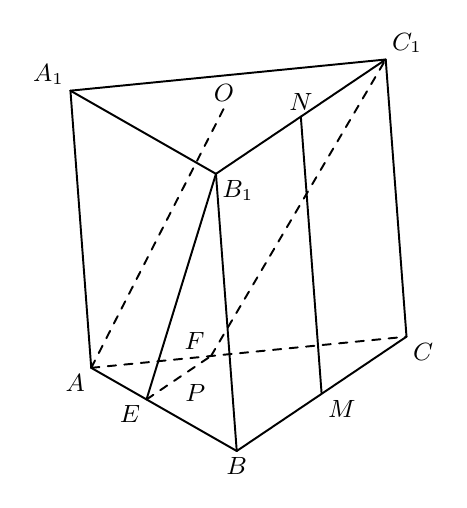
\begin{tikzpicture}[line width=0.7pt, font=\small,
  x=0.88cm, y=0.88cm, line cap=round, line join=round]
  % 底面 ABC 与上底面 A1B1C1 的平行投影
  \coordinate (A)  at (1.75,1.20);
  \coordinate (B)  at (3.85,0.00);
  \coordinate (C)  at (6.30,1.65);
  \coordinate (A1) at (1.45,5.20);
  \coordinate (B1) at (3.55,4.00);
  \coordinate (C1) at (6.00,5.65);
  % 中点、中心与截面相关点
  \coordinate (M)  at (5.075,0.825);
  \coordinate (N)  at (4.775,4.825);
  \coordinate (O)  at (3.667,4.950);
  \coordinate (P)  at (3.014,1.058);
  \coordinate (E)  at (2.548,0.744);
  \coordinate (F)  at (3.479,1.371);

  % 可见棱
  \draw (A1) -- (A);
  \draw (A1) -- (B1);
  \draw (A1) -- (C1);
  \draw (B1) -- (C1);
  \draw (C1) -- (C);
  \draw (C)  -- (B);
  \draw (B)  -- (A);
  \draw (B1) -- (B);
  % 中位线与截面可见边
  \draw (N) -- (M);
  \draw (B1) -- (E);

  % 被遮挡的棱与内部辅助线
  \draw[dashed] (A) -- (C);
  \draw[dashed] (A) -- (O);
  \draw[dashed] (E) -- (F);
  \draw[dashed] (F) -- (C1);

  % 顶点标注
  \node[above left,  inner sep=2pt] at (A1) {$A_1$};
  \node[below left,  inner sep=2pt] at (A)  {$A$};
  \node[below,       inner sep=2pt] at (B)  {$B$};
  \node[below right, inner sep=2pt] at (C)  {$C$};
  \node[above right, inner sep=2pt] at (C1) {$C_1$};
  \node[below right, inner sep=2pt] at (B1) {$B_1$};
  \node[above,       inner sep=2pt] at (N)  {$N$};
  \node[above,       inner sep=2pt] at (O)  {$O$};
  \node[below right, inner sep=2pt] at (M)  {$M$};
  \node[below left,  inner sep=2pt] at (E)  {$E$};
  \node[above left,  inner sep=2pt] at (F)  {$F$};
  \node[below right, inner sep=2pt] at (P)  {$P$};
\end{tikzpicture}
\end{center}
\nopagebreak[4]
\Needspace{4\baselineskip}
\textbf{解析}

\gksubpart{（1）}

\Needspace{5\baselineskip}
三棱柱中 $AA_1\parallel BB_1$；又 $BB_1C_1C$ 是矩形，$BB_1\parallel CC_1$。$M$，$N$ 分别是 $BC$，$B_1C_1$ 的中点，而 $BB_1C_1C$ 为平行四边形，故
\nopagebreak[4]
\[MN\parallel BB_1\parallel AA_1 .\]

\Needspace{5\baselineskip}
因为 $\triangle ABC$ 是正三角形、$M$ 是 $BC$ 的中点，所以
\nopagebreak[4]
\[AM\perp BC .\]
\Needspace{5\baselineskip}
又 $BB_1C_1C$ 是矩形，故 $BB_1\perp BC$；而 $MN\parallel BB_1$，所以
\nopagebreak[4]
\[MN\perp BC .\]
\Needspace{5\baselineskip}
$AM$ 与 $MN$ 是平面 $A_1AMN$ 内两条相交直线（交于 $M$），于是
\nopagebreak[4]
\[BC\perp\text{\text{平面} }A_1AMN .\]
\Needspace{5\baselineskip}
三棱柱中 $B_1C_1\parallel BC$，故 $B_1C_1\perp$ 平面 $A_1AMN$。而 $B_1C_1\subset$ 平面 $EB_1C_1F$，所以
\nopagebreak[4]
\[\text{\text{平面} }A_1AMN\perp\text{\text{平面} }EB_1C_1F .\]

\gksubpart{（2）}

由（1）知 $AM\perp BC$，$MN\perp BC$，且 $MN\parallel BB_1$。以 $M$ 为原点，$MB$ 所在直线为 $x$ 轴，$MA$ 所在直线为 $y$ 轴，过 $M$ 且平行于 $BB_1$ 的直线为 $z$ 轴，建立空间直角坐标系。

\Needspace{5\baselineskip}
不妨设 $AB=2$，则
\nopagebreak[4]
\[B(1,0,0),\quad C(-1,0,0),\quad A(0,\sqrt3,0),\quad M(0,0,0).\]
\Needspace{5\baselineskip}
设 $BB_1=(0,m,h)$（$h>0$，由 $BB_1\perp BC$ 知 $x$ 分量为 $0$），则
\nopagebreak[4]
\[B_1(1,m,h),\quad C_1(-1,m,h),\quad A_1(0,\sqrt3+m,h),\]
\Needspace{5\baselineskip}
$N$ 为 $B_1C_1$ 的中点，$N(0,m,h)$；$O$ 为 $\triangle A_1B_1C_1$ 的中心，
\nopagebreak[4]
\[O\left(0,\ \frac{\sqrt3+m+m+m}3,\ h\right)=\left(0,\ \frac{\sqrt3}3+m,\ h\right).\]
平面 $A_1AMN$ 即 $x=0$（$yz$ 平面）。

\Needspace{5\baselineskip}
设 $P(0,t\sqrt3,0)$（$0<t<1$）。平面 $EB_1C_1F$ 过直线 $B_1C_1$（方向 $(1,0,0)$）与点 $P$，其法向量可取
\nopagebreak[4]
\[\boldsymbol n=(1,0,0)\times\overrightarrow{PB_1}=(1,0,0)\times(1,\ m-t\sqrt3,\ h)=\left(0,\ -h,\ m-t\sqrt3\right),\]
\Needspace{5\baselineskip}
故平面方程为
\nopagebreak[4]
\[-h\left(y-t\sqrt3\right)+\left(m-t\sqrt3\right)z=0 .\]
令 $z=0$ 得 $y=t\sqrt3$，即该平面与底面 $ABC$ 的交线为 $y=t\sqrt3$（与 $BC$ 平行），这与「交 $AB$ 于 $E$、交 $AC$ 于 $F$」一致。

\Needspace{5\baselineskip}
由 $AO\parallel$ 平面 $EB_1C_1F$ 得 $\overrightarrow{AO}\cdot\boldsymbol n=0$，而
\nopagebreak[4]
\[\overrightarrow{AO}=\left(0,\ \frac{\sqrt3}3+m-\sqrt3,\ h\right)=\left(0,\ m-\frac{2\sqrt3}3,\ h\right),\]
\Needspace{5\baselineskip}
故
\nopagebreak[4]
\[-h\left(m-\frac{2\sqrt3}3\right)+h\left(m-t\sqrt3\right)=0\ \Longrightarrow\ t\sqrt3=\frac{2\sqrt3}3\ \Longrightarrow\ t=\frac23 .\]
\Needspace{5\baselineskip}
于是 $E$ 在 $AB$ 上满足 $y_E=t\sqrt3=\dfrac{2\sqrt3}3$。由 $A(0,\sqrt3,0)$、$B(1,0,0)$ 得
\nopagebreak[4]
\[E\left(\frac13,\ \frac{2\sqrt3}3,\ 0\right),\qquad F\left(-\frac13,\ \frac{2\sqrt3}3,\ 0\right).\]

\Needspace{5\baselineskip}
又 $AO=AB=2$，即
\nopagebreak[4]
\[\left(m-\frac{2\sqrt3}3\right)^2+h^2=4 .\]
\Needspace{5\baselineskip}
于是
\nopagebreak[4]
\[\overrightarrow{B_1E}=\left(\frac13-1,\ \frac{2\sqrt3}3-m,\ -h\right)=\left(-\frac23,\ -\left(m-\frac{2\sqrt3}3\right),\ -h\right),\]
\nopagebreak[4]
\[|\overrightarrow{B_1E}|=\sqrt{\frac49+\left(m-\frac{2\sqrt3}3\right)^2+h^2}=\sqrt{\frac49+4}=\frac{2\sqrt{10}}3 .\]
\Needspace{5\baselineskip}
平面 $A_1AMN$ 的法向量为 $(1,0,0)$，设直线 $B_1E$ 与平面 $A_1AMN$ 所成角为 $\theta$，则
\nopagebreak[4]
\[\sin\theta=\frac{\left|\overrightarrow{B_1E}\cdot(1,0,0)\right|}{|\overrightarrow{B_1E}|\cdot1}
=\frac{\frac23}{\frac{2\sqrt{10}}3}=\frac1{\sqrt{10}}=\frac{\sqrt{10}}{10} .\]

\gkanswer{答案（1）：证明。$MN\parallel BB_1\parallel AA_1$；又 $BC\perp AM$、$BC\perp MN$，故 $BC\perp$ 平面 $A_1AMN$，而 $B_1C_1\parallel BC$ 且 $B_1C_1\subset$ 平面 $EB_1C_1F$，故两平面垂直。}

\gkanswer{答案（2）：$\dfrac{\sqrt{10}}{10}$。以 $M$ 为原点、$MA$ 为 $y$ 轴、$MB$ 为 $x$ 轴建系，由 $AO\parallel$ 平面 $EB_1C_1F$ 与 $AO=AB$ 得 $|B_1E|=\dfrac{\sqrt{10}}3AB$、$B_1E$ 的横向分量为 $\dfrac13AB$。}

\end{answer}
\begin{answer}
\gksolhead{21}{}

\textbf{题目}：

已知函数 $f(x)=\sin^2x\sin2x$。

（1） 讨论 $f(x)$ 在区间 $(0,\pi)$ 的单调性；

（2） 证明：$|f(x)|\leqslant\dfrac{3\sqrt3}8$；

（3） 设 $n\in\mathbf N^*$，证明：$\sin^2x\sin^22x\sin^24x\cdots\sin^22^nx\leqslant\dfrac{3^n}{4^n}$。

\Needspace{4\baselineskip}
\textbf{解析}

\gksubpart{（1）}

\Needspace{5\baselineskip}
由 $\sin2x=2\sin x\cos x$ 得
\nopagebreak[4]
\[f(x)=2\sin^3x\cos x,\]
\Needspace{5\baselineskip}
求导：
\nopagebreak[4]
\[f'(x)=6\sin^2x\cos^2x-2\sin^4x=2\sin^2x\left(3\cos^2x-\sin^2x\right)=2\sin^2x\left(4\cos^2x-1\right).\]
\Needspace{5\baselineskip}
当 $x\in(0,\pi)$ 时 $\sin x>0$，故 $f'(x)$ 的符号由 $4\cos^2x-1$ 决定：
\nopagebreak[4]
\[f'(x)=0\iff \cos x=\pm\frac12\iff x=\frac\pi3\ \text{\text{或}}\ x=\frac{2\pi}3 .\]
列表：

\begin{center}
\begin{tabular}{llllll}
\toprule
$x$ & $\left(0,\dfrac\pi3\right)$ & $\dfrac\pi3$ & $\left(\dfrac\pi3,\dfrac{2\pi}3\right)$ & $\dfrac{2\pi}3$ & $\left(\dfrac{2\pi}3,\pi\right)$ \\
\midrule
$f'(x)$ & $+$ & $0$ & $-$ & $0$ & $+$ \\
$f(x)$ & 递增 & 极大值 & 递减 & 极小值 & 递增 \\
\bottomrule
\end{tabular}
\end{center}

所以 $f(x)$ 在 $\left(0,\dfrac\pi3\right)$ 与 $\left(\dfrac{2\pi}3,\pi\right)$ 上单调递增，在 $\left(\dfrac\pi3,\dfrac{2\pi}3\right)$ 上单调递减。

\gksubpart{（2）}

\Needspace{5\baselineskip}
由（1），$f$ 在 $[0,\pi]$ 上的最大值与最小值分别为
\nopagebreak[4]
\[f\left(\frac\pi3\right)=\sin^2\frac\pi3\sin\frac{2\pi}3=\frac34\cdot\frac{\sqrt3}2=\frac{3\sqrt3}8,\]
\nopagebreak[4]
\[f\left(\frac{2\pi}3\right)=\sin^2\frac{2\pi}3\sin\frac{4\pi}3=\frac34\cdot\left(-\frac{\sqrt3}2\right)=-\frac{3\sqrt3}8 .\]
\Needspace{5\baselineskip}
又 $f(0)=f(\pi)=0$，故对 $x\in[0,\pi]$ 有
\nopagebreak[4]
\[|f(x)|\leqslant\frac{3\sqrt3}8 .\]
\Needspace{5\baselineskip}
而 $f(x+\pi)=\sin^2(x+\pi)\sin(2x+2\pi)=\sin^2x\sin2x=f(x)$，即 $f$ 以 $\pi$ 为周期，故对一切 $x\in\mathbf R$ 都有
\nopagebreak[4]
\[|f(x)|\leqslant\frac{3\sqrt3}8 .\]

\gksubpart{（3）}

\Needspace{5\baselineskip}
记 $b_k=\left|\sin\left(2^kx\right)\right|$（$k=0,1,\cdots,n$）。由（2），对 $k=0,1,\cdots,n-1$ 都有
\nopagebreak[4]
\[b_k^2b_{k+1}=\sin^2\left(2^kx\right)\left|\sin\left(2^{k+1}x\right)\right|\leqslant\frac{3\sqrt3}8 .\]
\Needspace{5\baselineskip}
把这 $n$ 个不等式相乘，注意 $b_1,\cdots,b_{n-1}$ 各出现三次、$b_0$ 出现两次、$b_n$ 出现一次：
\nopagebreak[4]
\[b_0^2b_n\prod_{k=1}^{n-1}b_k^3\leqslant\left(\frac{3\sqrt3}8\right)^n .\]
\Needspace{5\baselineskip}
另一方面
\nopagebreak[4]
\[\left(\prod_{k=0}^{n}b_k^2\right)^{\frac32}=\prod_{k=0}^{n}b_k^3=b_0b_n^2\cdot b_0^2b_n\prod_{k=1}^{n-1}b_k^3
\leqslant b_0b_n^2\left(\frac{3\sqrt3}8\right)^n\leqslant\left(\frac{3\sqrt3}8\right)^n,\]
\Needspace{5\baselineskip}
其中最后一步用了 $0\leqslant b_0\leqslant1$、$0\leqslant b_n\leqslant1$。于是
\nopagebreak[4]
\[\prod_{k=0}^{n}\sin^2\left(2^kx\right)=\prod_{k=0}^{n}b_k^2\leqslant\left(\frac{3\sqrt3}8\right)^{\frac{2n}3} .\]
\Needspace{5\baselineskip}
最后化简常数：
\nopagebreak[4]
\[\left(\frac{3\sqrt3}8\right)^{\frac23}=\frac{\left(3\sqrt3\right)^{\frac23}}{8^{\frac23}}=\frac{27^{\frac13}}{4}=\frac34,\]
\Needspace{5\baselineskip}
故
\nopagebreak[4]
\[\sin^2x\sin^22x\sin^24x\cdots\sin^22^nx\leqslant\left(\frac34\right)^n=\frac{3^n}{4^n} .\]

\gkanswer{答案（1）：在 $\left(0,\dfrac\pi3\right)$、$\left(\dfrac{2\pi}3,\pi\right)$ 单调递增，在 $\left(\dfrac\pi3,\dfrac{2\pi}3\right)$ 单调递减。由 $f'(x)=2\sin^2x(4\cos^2x-1)$ 定号。}

\gkanswer{答案（2）：证明。$f$ 在 $[0,\pi]$ 上的最大值为 $f\left(\dfrac\pi3\right)=\dfrac{3\sqrt3}8$，最小值为 $f\left(\dfrac{2\pi}3\right)=-\dfrac{3\sqrt3}8$，且 $f$ 以 $\pi$ 为周期。}

\gkanswer{答案（3）：证明。记 $b_k=|\sin2^kx|$，由（2）得 $b_k^2b_{k+1}\leqslant\dfrac{3\sqrt3}8$（$k=0,\cdots,n-1$），连乘后与 $\prod b_k^3$ 比较，得 $\prod b_k^2\leqslant\left(\dfrac{3\sqrt3}8\right)^{2n/3}=\left(\dfrac34\right)^n$。}

\end{answer}
\begin{answer}
\gksolhead{22}{【A】选修 4—4：坐标系与参数方程}

\textbf{题目}【A】（选修 4—4：坐标系与参数方程）：

已知曲线 $C_1$，$C_2$ 的参数方程分别为 $C_1:\begin{cases}x=4\cos^2\theta,\\y=4\sin^2\theta\end{cases}$（$\theta$ 为参数），$C_2:\begin{cases}x=t+\dfrac1t,\\y=t-\dfrac1t\end{cases}$（$t$ 为参数）。

（1） 将 $C_1$，$C_2$ 的参数方程化为普通方程；

（2） 以坐标原点为极点，$x$ 轴正半轴为极轴建立极坐标系。设 $C_1$，$C_2$ 的交点为 $P$，求圆心在极轴上，且经过极点和 $P$ 的圆的极坐标方程。

\Needspace{4\baselineskip}
\textbf{解析}

\gksubpart{（1）}

\Needspace{5\baselineskip}
对 $C_1$：由 $x=4\cos^2\theta$，$y=4\sin^2\theta$ 相加得
\nopagebreak[4]
\[x+y=4,\]
\Needspace{5\baselineskip}
又 $\cos^2\theta\in[0,1]$，故 $0\leqslant x\leqslant4$，$0\leqslant y\leqslant4$。所以 $C_1$ 的普通方程为
\nopagebreak[4]
\[x+y=4\quad(0\leqslant x\leqslant4),\]
即连接 $(4,0)$ 与 $(0,4)$ 的线段。

\Needspace{5\baselineskip}
对 $C_2$：由 $x=t+\dfrac1t$，$y=t-\dfrac1t$ 得
\nopagebreak[4]
\[x^2-y^2=\left(t+\frac1t\right)^2-\left(t-\frac1t\right)^2=4,\]
\Needspace{5\baselineskip}
所以 $C_2$ 的普通方程为
\nopagebreak[4]
\[x^2-y^2=4 .\]

\gksubpart{（2）}

\Needspace{5\baselineskip}
把 $C_1$ 的方程写成 $x+y=4$，与 $C_2$ 的方程联立：
\nopagebreak[4]
\[x^2-y^2=(x+y)(x-y)=4\ \Longrightarrow\ 4(x-y)=4\ \Longrightarrow\ x-y=1 .\]
\Needspace{5\baselineskip}
解得
\nopagebreak[4]
\[x=\frac52,\qquad y=\frac32,\]
即交点 $P\left(\dfrac52,\dfrac32\right)$（满足 $0\leqslant x\leqslant4$，确在 $C_1$ 的线段上）。

\Needspace{5\baselineskip}
设所求圆的圆心为 $(a,0)$（圆心在极轴上）。圆过极点 $O$，故半径 $r=|a|$；又圆过 $P$，故
\nopagebreak[4]
\[\left(\frac52-a\right)^2+\left(\frac32\right)^2=a^2 .\]
\Needspace{5\baselineskip}
展开得
\nopagebreak[4]
\[\frac{25}4-5a+a^2+\frac94=a^2\ \Longrightarrow\ 5a=\frac{34}4=\frac{17}2\ \Longrightarrow\ a=\frac{17}{10}>0 .\]
\Needspace{5\baselineskip}
以极点为圆心在极轴上的圆，其极坐标方程为 $\rho=2a\cos\theta$，故
\nopagebreak[4]
\[\rho=\frac{17}5\cos\theta .\]

\gkanswer{答案（1）：$C_1:x+y=4$（$0\leqslant x\leqslant4$），$C_2:x^2-y^2=4$。前者由 $4\cos^2\theta+4\sin^2\theta=4$ 消参，后者由 $x^2-y^2=4$ 消参。}

\gkanswer{答案（2）：$\rho=\dfrac{17}5\cos\theta$。交点 $P\left(\dfrac52,\dfrac32\right)$，圆心 $\left(\dfrac{17}{10},0\right)$，故 $\rho=2\cdot\dfrac{17}{10}\cos\theta$。}

\end{answer}
\begin{answer}
\gksolhead{23}{【B】选修 4—5：不等式选讲}

\textbf{题目}【B】（选修 4—5：不等式选讲）：

已知函数 $f(x)=|x-a^2|+|x-2a+1|$。

（1） 当 $a=2$ 时，求不等式 $f(x)\geqslant4$ 的解集；

（2） 若 $f(x)\geqslant4$，求 $a$ 的取值范围。

\Needspace{4\baselineskip}
\textbf{解析}

\gksubpart{（1）}

\Needspace{5\baselineskip}
当 $a=2$ 时，
\nopagebreak[4]
\[f(x)=|x-4|+|x-3| .\]
分段讨论：

当 $x\leqslant3$ 时，$f(x)=(4-x)+(3-x)=7-2x$，由 $7-2x\geqslant4$ 得 $x\leqslant\dfrac32$；

当 $3<x<4$ 时，$f(x)=(4-x)+(x-3)=1$，不满足 $f(x)\geqslant4$；

当 $x\geqslant4$ 时，$f(x)=(x-4)+(x-3)=2x-7$，由 $2x-7\geqslant4$ 得 $x\geqslant\dfrac{11}2$。

\Needspace{5\baselineskip}
故解集为
\nopagebreak[4]
\[\left(-\infty,\frac32\right]\cup\left[\frac{11}2,+\infty\right).\]

\gksubpart{（2）}

\Needspace{5\baselineskip}
对任意 $x$，
\nopagebreak[4]
\[f(x)=|x-a^2|+|x-(2a-1)|\geqslant\left|a^2-(2a-1)\right|=(a-1)^2,\]
且当 $x$ 介于 $a^2$ 与 $2a-1$ 之间时取到等号（由 $a^2-(2a-1)=(a-1)^2\geqslant0$ 知这段区间非空，故最小值确能取到）。

\Needspace{5\baselineskip}
题设「$f(x)\geqslant4$」按「对任意 $x$ 恒成立」理解，等价于最小值不小于 $4$：
\nopagebreak[4]
\[(a-1)^2\geqslant4\ \Longrightarrow\ |a-1|\geqslant2 .\]
\Needspace{5\baselineskip}
解得
\nopagebreak[4]
\[a-1\geqslant2\ \text{\text{或}}\ a-1\leqslant-2,\]
\Needspace{5\baselineskip}
即
\nopagebreak[4]
\[a\geqslant3\ \text{\text{或}}\ a\leqslant-1 .\]
\Needspace{5\baselineskip}
故 $a$ 的取值范围为
\nopagebreak[4]
\[(-\infty,-1]\cup[3,+\infty).\]

\gkanswer{答案（1）：$\left(-\infty,\dfrac32\right]\cup\left[\dfrac{11}2,+\infty\right)$。$a=2$ 时 $f(x)=|x-4|+|x-3|$，分段求解 $f(x)\geqslant4$。}

\gkanswer{答案（2）：$a\leqslant-1$ 或 $a\geqslant3$。$f(x)$ 的最小值为 $(a-1)^2$，故 $(a-1)^2\geqslant4$。}

\end{answer}